\documentclass[11pt,a4paper]{article}
\usepackage[margin=23mm,headheight=16pt]{geometry}
\usepackage[T1]{fontenc}\usepackage{tgpagella}\usepackage{amsmath,amssymb,amsthm,mathtools,bm,mathrsfs,microtype,booktabs,tabularx,longtable,enumitem,graphicx}
\usepackage{tikz}\usetikzlibrary{arrows.meta,positioning,calc}
\usepackage{xcolor,fancyhdr,hyperref}\definecolor{deepblue}{RGB}{25,50,99}\definecolor{purple}{RGB}{104,69,170}\definecolor{softblue}{RGB}{227,238,249}
\hypersetup{colorlinks=true,linkcolor=deepblue,urlcolor=deepblue}\pagestyle{fancy}\fancyhf{}\fancyhead[L]{\small Quantum Measurement, Feedback and Correction}\fancyhead[R]{\small Companion VIII}\fancyfoot[C]{\thepage}\emergencystretch=1em\setlength{\parskip}{5pt}\setlength{\parindent}{0pt}\setcounter{secnumdepth}{3}
\newtheorem{example}{Worked Example}\newtheorem{remark}{Qualification}\newtheorem{proposition}{Proposition}
\newcommand{\tr}{\operatorname{Tr}}\newcommand{\D}{\mathcal D}\newcommand{\ket}[1]{|#1\rangle}\newcommand{\bra}[1]{\langle#1|}\newcommand{\E}{\mathbb E}\newcommand{\ip}[2]{\langle#1|#2\rangle}
\begin{document}
\begin{center}
{\Large\bfseries\color{deepblue} Quantum Measurement-Induced Transitions,\\ Feedback and Error Correction in Rubidium Lattices}\par\medskip
{\large Chapter VIII --- exact diagonalization, monitored trajectories,\\ entanglement, reservoir engineering and quantum codes}\par\smallskip
{\small Rubidium-87 Quantum Physics Companion --- append-only continuation of Chapters I--VII}\par
\end{center}
\begin{abstract}
This chapter extends the prior discussion of Lindblad evolution into independently reproducible numerical quantum trajectories, trajectory-resolved bipartite entropy, finite-size monitoring crossovers, measurement-based feedback, and engineered dissipative preparation. A two-site/two-boson Bose--Hubbard dimer is diagonalized analytically and evolved numerically with $1200$ jump trajectories per monitoring strength; their ensemble density matrices are compared to direct exponentiation of the nine-dimensional Lindblad superoperator. We distinguish spatial-mode entanglement from particle entanglement, the conditional from the unconditional state, finite-size crossovers from thermodynamic measurement-induced transitions, and preparation of a known target from autonomous quantum error correction of unknown encoded information. Numerical data, plots and executable Python are supplied as companion files. No claim is made that the model represents an actual realization of this monitoring and feedback protocol on Tiangong.
\end{abstract}
\tableofcontents\clearpage
\section{The physical and mathematical setting}
In a dilute ultracold rubidium lattice, the degrees of freedom in the Bose--Hubbard description refer to \emph{whole atoms in Wannier motional orbitals}. The internal atomic electronic state remains approximately frozen within a selected hyperfine manifold. For a short open chain, the standard model is
\begin{equation}\label{eq:bh}
H_{\rm BH}=-J\sum_{\langle i,j\rangle}(a_i^\dagger a_j+a_j^\dagger a_i)+\frac U2\sum_i n_i(n_i-1)+\sum_i V_i n_i.
\end{equation}
An idealized local number-monitoring channel is represented by $L_i=\sqrt\gamma\,n_i$. The unconditional Markovian evolution is
\begin{equation}\label{eq:lind}
\boxed{\dot\rho=-\frac{i}{\hbar}[H_{\rm BH},\rho]+\gamma\sum_i\D[n_i]\rho,\qquad \D[L]\rho=L\rho L^\dagger-\tfrac12\{L^\dagger L,\rho\}.}
\end{equation}
This local-density model is a controlled theoretical description rather than a universal model of fluorescence; real experiments can involve recoil, imperfect collection, parity-limited imaging, state-changing scattering, and loss. Conditioned dynamics depends on the \emph{measurement instrument}, not solely the average Lindbladian.
\begin{figure}[ht]\centering
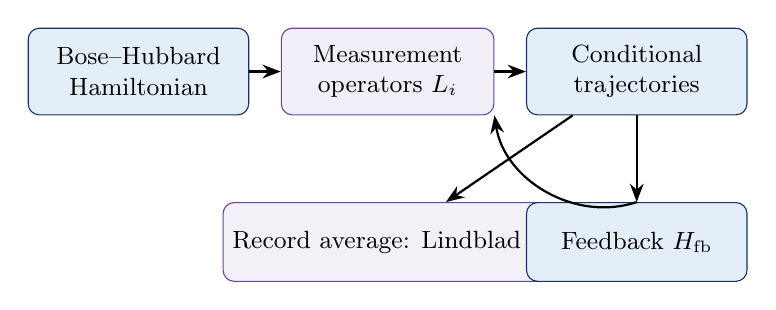
\begin{tikzpicture}[>=Stealth,node distance=4mm,every node/.style={font=\small}]
\node[draw=deepblue,fill=softblue,rounded corners,minimum width=2.8cm,minimum height=11mm,align=center] (h) {Bose--Hubbard\\Hamiltonian};
\node[draw=purple,fill=purple!9,rounded corners,minimum width=2.7cm,minimum height=11mm,align=center,right=of h] (m) {Measurement\\operators $L_i$};
\node[draw=deepblue,fill=softblue,rounded corners,minimum width=2.8cm,minimum height=11mm,align=center,right=of m] (t) {Conditional\\trajectories};
\draw[->,thick] (h)--(m);\draw[->,thick] (m)--(t);
\node[draw=purple,fill=purple!8,rounded corners,below=11mm of m,align=center,minimum width=3.8cm,minimum height=10mm] (e) {Record average: Lindblad $\rho$};
\node[draw=deepblue,fill=softblue,rounded corners,below=11mm of t,align=center,minimum width=2.8cm,minimum height=10mm] (f) {Feedback $H_{\rm fb}$};
\draw[->,thick] (t)--(e);\draw[->,thick] (t)--(f);\draw[->,thick,bend left=50] (f.north) to (m.south east);
\end{tikzpicture}
\caption{An observation record resolves a conditional stochastic state; averaging the same record ensemble reconstructs the unconditional density matrix. A controller acts on the conditioned estimate, with efficacy limited by bandwidth, inefficiency and physical controls.}
\end{figure}
\section{The exactly solvable two-site problem}
With two bosons on two sites, use the Fock basis $\mathcal B=(\ket{20},\ket{11},\ket{02})$. The matrix is
\begin{equation}\label{eq:H}
H=\begin{pmatrix}U&-\sqrt2J&0\\-\sqrt2J&0&-\sqrt2J\\0&-\sqrt2J&U\end{pmatrix}.
\end{equation}
Define $\ket{S}=(\ket{20}+\ket{02})/\sqrt2$ and $\ket{A}=(\ket{20}-\ket{02})/\sqrt2$. The antisymmetric state has energy $U$, while the symmetric block has matrix $\bigl(\begin{smallmatrix}U&-2J\\-2J&0\end{smallmatrix}\bigr)$ and eigenenergies
\begin{equation}\label{eq:spectrum}E_\pm=\frac{U\pm\sqrt{U^2+16J^2}}2,\qquad E_A=U.\end{equation}
\begin{example}[Exact numerical eigenvalues]
Set $\hbar=J=1$ and $U=4$. Then $E_- =2-2\sqrt2=-0.82842712$, $E_A=4$, $E_+=2+2\sqrt2=4.82842712$. This is an exact-diagonalization benchmark: the numerical eigensolver must reproduce all three and orthonormal eigenvectors.
\end{example}
\begin{example}[Initial coherent two-boson state]
Use $\ket{\psi_0}=\frac12\ket{20}+\frac1{\sqrt2}\ket{11}+\frac12\ket{02}$. It is the $U=0$ bonding-orbital state and has $\langle n_L\rangle=\langle n_R\rangle=1$, $P_{11}=1/2$. Its spatial-mode Schmidt probabilities are $(1/4,1/2,1/4)$, giving $S_L(0)=\tfrac32\ln2=1.03972077$ nats.
\end{example}
\section{Local number monitoring and its decoherence rate}
The site-number matrices in $\mathcal B$ are
\begin{equation}
n_L=\operatorname{diag}(2,1,0),\qquad n_R=\operatorname{diag}(0,1,2),\quad L_{L,R}=\sqrt\gamma\,n_{L,R}.
\end{equation}
The dissipator acts on the matrix element between Fock configurations $\ket{\mathbf n}$ and $\ket{\mathbf m}$ as
\begin{equation}\label{eq:dephase}
\left.\frac{d\rho_{\mathbf n\mathbf m}}{dt}\right|_{\rm monitor}=-\frac\gamma2\sum_i(n_i-m_i)^2\rho_{\mathbf n\mathbf m}.
\end{equation}
This holds because $n_i$ is Hermitian and diagonal in the occupation basis.
\begin{example}[Distinct dephasing channels]
For the $\ket{20}\!\bra{11}$ coherence, the occupations differ by $(1,-1)$; its monitoring-only decay rate is $\gamma$. For $\ket{20}\!\bra{02}$ the difference is $(2,-2)$ and the decay rate is $4\gamma$. Thus a measurement that resolves a larger occupation difference causes faster decay of the associated coherences.
\end{example}
\begin{remark}
The operators $\sqrt\gamma n_L$ and $\sqrt\gamma n_R$ are a particular jump unraveling, and can generate ``click'' records with state-dependent event intensities. A diffusive (homodyne-like) unraveling of the same GKSL generator produces different individual conditioned paths. The ensemble density matrix is the invariant comparison target.
\end{remark}
\section{Quantum-jump evolution and statistical reconstruction}
For normalized $\ket\psi$ and timestep $dt$, the monitored channel probabilities are
\begin{equation}p_\mu=dt\,\bra\psi L_\mu^\dagger L_\mu\ket\psi,\quad H_{\rm eff}=H-\frac{i\hbar}2\sum_\mu L_\mu^\dagger L_\mu.\end{equation}
If a jump occurs, $\ket\psi\to L_\mu\ket\psi/\|L_\mu\ket\psi\|$. Otherwise $\ket\psi\to e^{-iH_{\rm eff}dt/\hbar}\ket\psi$ followed by normalization. The timestep must ensure $\sum p_\mu\ll1$, otherwise multi-event corrections and discretization effects become significant. The estimator is
\begin{equation}\label{eq:rhomc}\rho_{\rm MC}(t)=\frac1{N_{\rm tr}}\sum_{r=1}^{N_{\rm tr}}\ket{\psi_r(t)}\bra{\psi_r(t)}.\end{equation}
The benchmark computes an independent exact matrix exponential of the Lindblad \emph{superoperator} on the vectorized $3\times3$ density matrix. In column-major convention,
\begin{equation}\label{eq:liouv}
\mathscr L_H=-i(I\otimes H-H^{\mathsf T}\otimes I),\quad\mathscr L_L=L^*\otimes L-\tfrac12(I\otimes L^\dagger L+(L^\dagger L)^\mathsf T\otimes I).
\end{equation}
For $\hbar=1$, the exact master solution is $\operatorname{vec}\rho(t)=e^{t\mathscr L}\operatorname{vec}\rho(0)$.
\begin{example}[Reproducible numerical protocol]
The included \texttt{simulate.py} uses $U/J=4$, timestep $dtJ/\hbar=0.005$, evolution to $Jt/\hbar=3$, and $1200$ trajectories per $\gamma/J\in\{0,0.5,2\}$. The pseudo-random seed is $20261118$. Sampling and timestep errors are reported, never concealed. Under this setup the largest observed sampled-matrix Frobenius discrepancy is approximately $0.0332$.
\end{example}
\begin{table}[ht]\centering\small
\caption{Independent master-equation and Monte Carlo results at $Jt/\hbar=3$. MC contains 1200 trajectories per condition.}
\begin{tabular}{@{}rrrrrr@{}}\toprule
$\gamma/J$ & $P_{11}^{\rm exact}$ & $P_{11}^{\rm MC}$ & $\overline{S_L}$ & $\tr\rho^2$ & $\|\rho_{\rm MC}-\rho\|_F$\\\midrule
0 & .825835 & .825835 & .583151 & 1.000000 & $<10^{-12}$\\
0.5 & .566301 & .565489 & .684820 & .465820 & .026873\\
2 & .371811 & .350567 & .462381 & .336833 & .033115\\\bottomrule
\end{tabular}
\end{table}
\begin{figure}[ht]\centering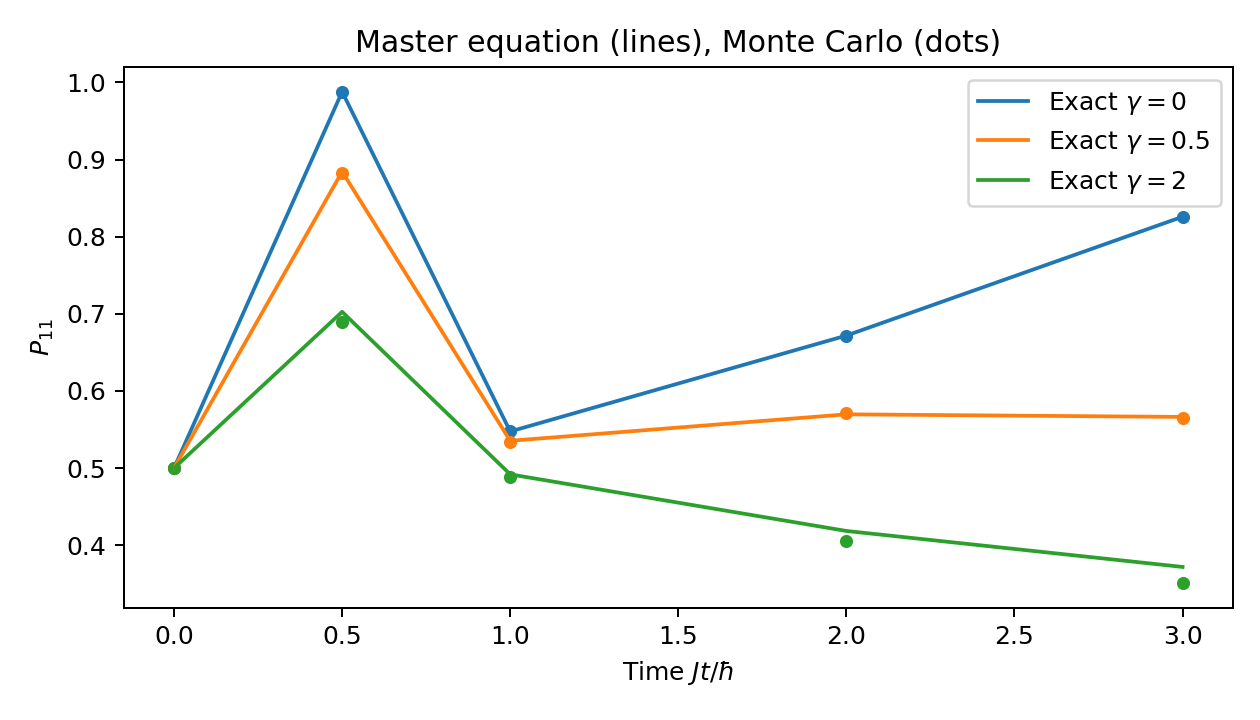
\includegraphics[width=.92\linewidth]{master_versus_trajectories.png}\caption{Exact Lindblad curves (lines) versus independently sampled jump trajectories (points). Scatter is finite-sample Monte Carlo error and a smaller time-discretization contribution.}\end{figure}
\clearpage
\section{Entanglement along a conditioned trajectory}
For a fixed-two-boson pure state $\ket\psi=c_{20}\ket{20}+c_{11}\ket{11}+c_{02}\ket{02}$, the reduced density matrix of the left site is diagonal, with probabilities $p=(|c_{02}|^2,|c_{11}|^2,|c_{20}|^2)$. The spatial-mode entropy is therefore
\begin{equation}\label{eq:ent}S_L(\psi)=-\sum_{n=0}^{2}p_n\ln p_n.\end{equation}
The monitored \emph{trajectory-average entropy} is $\bar S_L(t)=N_{\rm tr}^{-1}\sum_r S_L(\psi_r(t))$. By contrast, the unconditional master density matrix $\rho(t)$ may be mixed, and $S(\tr_R\rho)$ is not an entanglement entropy for that mixed global state.
\begin{example}[Nonlinearity of trajectory entropy]
Consider two equally likely, orthogonal pure trajectories $\ket{20}$ and $\ket{02}$. Each is a product of left/right number states, so the averaged trajectory entanglement is zero. The unconditional mixture $\tfrac12\ket{20}\bra{20}+\tfrac12\ket{02}\bra{02}$ has left reduced entropy $\ln2$. That entropy reflects classical uncertainty about the record, not entanglement of either trajectory.
\end{example}
\begin{example}[One run, three monitoring strengths]
At final time $Jt/\hbar=3$, the mean pure-trajectory spatial-mode entropies in our seeded simulation are $0.583151$ nats for $\gamma=0$, $0.684820$ for $\gamma/J=0.5$ and $0.462381$ for $\gamma/J=2$. They are neither monotonic in $\gamma$ at a fixed finite time nor universal: the unitary quench, jump timing and finite lattice all matter.
\end{example}
\begin{figure}[ht]\centering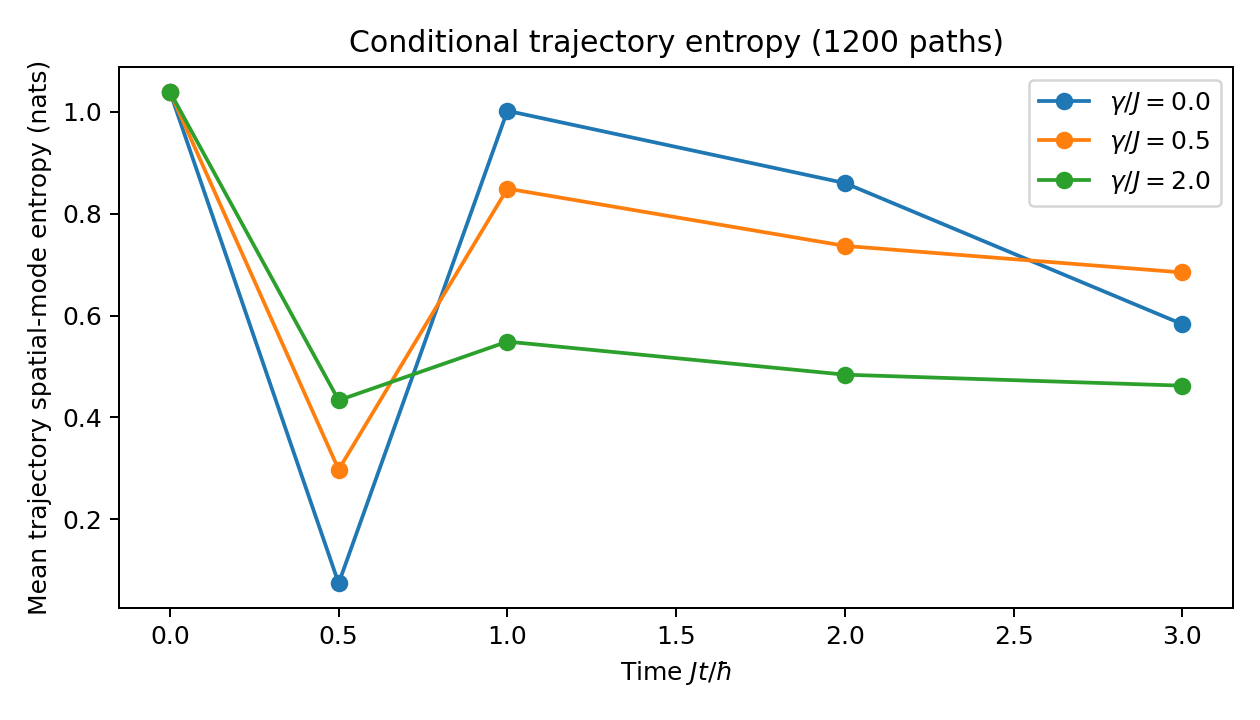
\includegraphics[width=.92\linewidth]{trajectory_entropy.png}\caption{Trajectory-averaged pure-state spatial-mode entropy. The plot describes a finite dimer at selected times; it is not a measurement-induced phase diagram.}\end{figure}
\section{What counts as a measurement-induced transition?}
A measurement-induced entanglement transition refers to a nonanalytic change in an appropriate large-system scaling limit of \emph{conditioned} states as a monitoring/control parameter changes. A robust claim requires (i) a family of increasing system sizes, (ii) a defined ensemble of measurement records, (iii) an entanglement or purification diagnostic, (iv) suitable long-time and sampling limits, and (v) finite-size scaling or related critical evidence.
A two-site calculation can demonstrate entanglement suppression, quantum Zeno dynamics, or a crossover, but \emph{not} establish a thermodynamic phase transition. Different monitored models may exhibit area-law, volume-law or other entanglement regimes; fixed particle number and conserved quantities may alter scaling. For a monitored Bose--Hubbard dimer, more specialized large-$N$ limits and transitions have been studied, but these are not implied by the present $N=2$ calculation.
\begin{remark}[Scaling and postselection]
Conditional entanglement can depend on the record. The probability of reproducing one detailed record typically shrinks rapidly as the number of measurement events increases. Averaging experimentally accessible observables is not automatically equivalent to averaging a nonlinear trajectory entanglement estimator.
\end{remark}
\section{Measurement-based feedback}
Suppose an experimental record $y_{[0,t]}$ is used to compute a conditional state estimate $\rho_c(t)$. A feedback controller can choose a physical control Hamiltonian $H_{\rm fb}[y_{[0,t]}]$ and modify the subsequent evolution:
\begin{equation}d\rho_c=\left[-\frac{i}{\hbar}[H+H_{\rm fb},\rho_c]+\sum_\mu\D[L_\mu]\rho_c\right]dt+\text{innovation terms}.\end{equation}
The actual stochastic master equation depends on whether the record is counting, homodyne or another continuous measurement, and on efficiency, feedback delay, bandwidth and actuator noise. An arbitrary state-dependent Hamiltonian cannot be substituted without specifying a physical controller and detection model.
\begin{example}[A simple classical-conditional decision]
Suppose a number-resolved measurement finds $\ket{20}$ rather than the target $\ket{11}$. A controllable tunnel coupling can move one atom toward the other well, but its action must be calibrated because bosonic tunneling couples both double-occupancy states to $\ket{11}$. A naive instantaneous ``corrective flip'' of occupation labels is not a physical unitary defined on the full three-state Hilbert space.
\end{example}
\section{Engineered dissipation and unique target-state preparation}
A mathematically transparent control primitive is an engineered jump operator that transfers an undesired state $\ket E$ into a desired target $\ket G$:
\begin{equation}\label{eq:prep}L_{\rm prep}=\sqrt\kappa\ket G\bra E,\qquad L_{\rm prep}\ket G=0.\end{equation}
For a two-level subspace spanned by $\ket G,\ket E$, assume $[H,\ket G\bra G]=0$ and no competing dissipator. Then
\begin{equation}\label{eq:fidelity}F_G(t)=\bra G\rho(t)\ket G=1-[1-F_G(0)]e^{-\kappa t}.\end{equation}
The target is a dark state, and population decays from $\ket E$ into $\ket G$. The model is exactly solvable; however, constructing such a many-body nonlocal jump from local optical addressing and dissipation requires separate engineering.
\begin{example}[Numerical preparation fidelity]
For $F_G(0)=0.25$ and $\kappa t=2$, equation \eqref{eq:fidelity} gives $F_G=1-0.75e^{-2}=0.898499$. At $\kappa t=5$, $F_G\approx0.994947$. The gap $\kappa$ controls the approach toward the target in this ideal two-level model.
\end{example}
\begin{proposition}[Dark-state criterion]
If a pure target $\ket G$ is simultaneously a (possibly phase-rotating) eigenstate of the Hamiltonian and a common dark state of all jump operators, then $\ket G\bra G$ is stationary. This does not by itself prove that it is the \emph{unique} stationary state or that the system converges to it from every initial condition; those properties require analysis of the full Liouvillian.
\end{proposition}

\subsection{A numerical reservoir-engineering benchmark}
To supplement the analytic formula, the companion \texttt{control\_tests.py} simulates 3000 independent quantum-jump preparation paths for the idealized two-state target model. The initial target probability is $F_G(0)=0.25$ and $\kappa=1$. If a run starts in the undesirable state, the first transfer event occurs after an exponential waiting time with mean $1/\kappa$. The fraction of trajectories reaching $\ket G$ by time $t$ estimates the exact Lindblad fidelity $1-0.75e^{-\kappa t}$.
\begin{figure}[ht]\centering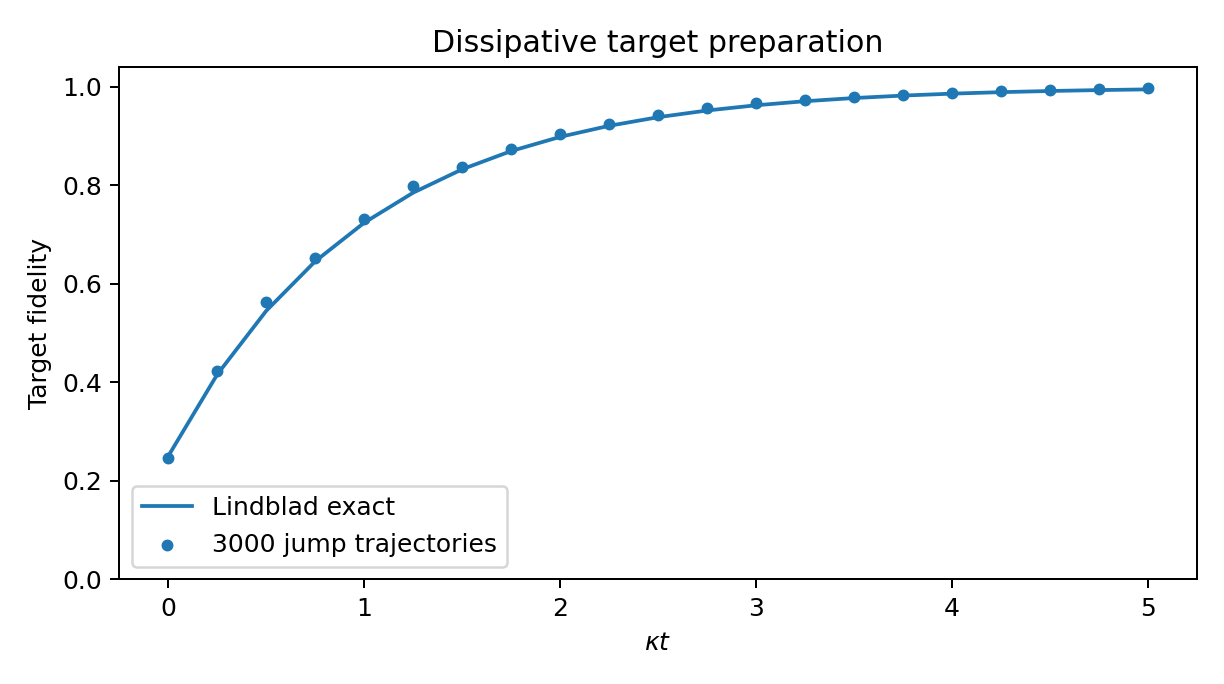
\includegraphics[width=.86\linewidth]{dissipative_preparation.png}\caption{Exact target-state fidelity versus an independent Monte Carlo preparation simulation (3000 paths). This is an abstract engineered-reservoir model, not an implementation of local Rb optical pumping.}\end{figure}
\begin{example}[Preparation accuracy and an important limitation]
At $\kappa t=2$ the exact target fidelity is $0.898499$. The source file records the Monte Carlo estimate. A system engineered to prepare one \emph{known} state need not preserve an unknown logical qubit; a single attractive pure state is not a quantum-memory code.
\end{example}

\section{Error correction is not merely state preparation}
To prepare a known state is to steer the apparatus toward one desired density matrix. Quantum error correction is more demanding: it must preserve an \emph{unknown} logical superposition $\alpha\ket{0_L}+\beta\ket{1_L}$ while correcting a specified error set.
For a code subspace with projector $P$ and candidate errors $E_a$, the Knill--Laflamme condition is
\begin{equation}\label{eq:KL}\boxed{PE_a^\dagger E_bP=c_{ab}P.}\end{equation}
This expresses the requirement that correctable error syndromes reveal nothing about the unknown logical amplitudes.
\begin{example}[Three physical qubits encoded in rubidium hyperfine states]
An abstract three-qubit bit-flip code uses $\ket{0_L}=\ket{000}$ and $\ket{1_L}=\ket{111}$. The stabilizer operators $Z_1Z_2$ and $Z_2Z_3$ detect a single $X_i$ error. The syndromes $(-,+)$, $(-,-)$, $(+,-)$ correspond to flips on qubits 1, 2 and 3 respectively. This code corrects one bit flip, but not arbitrary phase errors. Encoding and parity-readout gates in actual Rb hyperfine qubits require suitable coherent control; the abstract code does not establish experimental readiness.
\end{example}
\begin{example}[Why local number monitoring can damage a code]
The states $\ket{20}$ and $\ket{02}$ might be proposed as logical basis states. However, a measurement of $n_L$ perfectly distinguishes them. Such monitoring reveals the logical $Z$ value and dephases an unknown superposition of these states. Without a protected syndrome coupling or redundancy, this is not a nondestructive logical-error measurement.
\end{example}

\subsection{An explicit logical recovery test}
The included \texttt{control\_tests.py} constructs a nontrivial logical input $\ket{\psi_L}=\sqrt{0.37}\ket{000}+e^{0.63i}\sqrt{0.63}\ket{111}$, applies an $X_2$ error, evaluates the two stabilizer eigenvalues, and applies the corresponding correction. It obtains syndrome $(-1,-1)$ and final ideal state fidelity $1$ (to floating-point precision). This is an exact circuit-level algebraic check: noisy syndrome extraction, leakage, actuator constraints and fault tolerance are not included.
\begin{example}[Syndrome does not reveal amplitudes]
For the encoded state $\alpha\ket{000}+\beta\ket{111}$, a single $X_2$ error maps it to $\alpha\ket{010}+\beta\ket{101}$. Both terms have the same stabilizer eigenvalues $(-1,-1)$, so the syndrome identifies the error without measuring whether the logical state was $\ket{0_L}$ or $\ket{1_L}$. Applying $X_2$ restores the unknown coefficients $\alpha,\beta$.
\end{example}

\section{Validation and numerical limitations}
A credible numerical report should independently check $H^\dagger=H$, $\tr\rho=1$, positivity of exact $\rho(t)$, step-size stability, convergence with $N_{\rm tr}$, consistent vectorization conventions, and the distinction between pure-trajectory and mixed-state entropy. Our supplied script uses independent $3\times3$ Hamiltonian and $9\times9$ Liouvillian paths. The initial state, random seed, rates and time grid are explicit.
\begin{table}[ht]\centering\small
\caption{Validation ledger for this finite-size numerical chapter.}
\begin{tabularx}{\linewidth}{@{}lX@{}}\toprule
Check & Acceptance interpretation\\\midrule
Hermiticity & Analytic $H$ is real symmetric; eigenspectrum is real.\\
Trace & All reported Monte Carlo mean states have trace $1$ to numerical precision.\\
Master evolution & Matrix-exponential solution of the $9\times9$ Liouvillian is computed separately.\\
MC comparison & Maximum sampled Frobenius difference $\approx0.0332$ for 1200 trajectories per rate.\\
Purity & Exact Lindblad state has $\tr\rho^2\le1$; individual normalized jump states remain pure.\\
Limitations & No system-size scaling, continuous-detection efficiency model, or demonstration of an experimental QEC implementation.\\\bottomrule
\end{tabularx}
\end{table}
\section{Further worked derivations}
\begin{example}[Zeno estimate for a one-particle dimer]
For $H=-J\sigma_x$ and site monitoring that dephases the off-diagonal density matrix at rate $\gamma$, the Bloch imbalance obeys $\ddot z+\gamma\dot z+4J^2z/\hbar^2=0$. For $\gamma\gg J/\hbar$ the slow decay rate approaches $4J^2/(\hbar^2\gamma)$. More monitoring can suppress transport; it does not suppress all changes to every observable.
\end{example}
\begin{example}[Purity distinguishes unconditional mixing]
For the ideal one-particle balanced two-site density matrix $\rho(t)=\tfrac12\bigl(\begin{smallmatrix}1&e^{-\gamma t}\\e^{-\gamma t}&1\end{smallmatrix}\bigr)$, the purity is $\tr\rho^2=(1+e^{-2\gamma t})/2$. It decays from $1$ to $1/2$ as the unread which-site information accumulates.
\end{example}
\begin{example}[Finite-sample error scales]
For independent bounded scalar observables, standard Monte Carlo uncertainty typically falls as $N_{\rm tr}^{-1/2}$. Increasing from 1200 to 4800 trajectories should reduce sampling-dominated error by about a factor of two, but time discretization must also be reduced to rule out bias.
\end{example}
\begin{example}[Monitoring is not identical to particle loss]
$L_i=\sqrt\gamma n_i$ preserves total particle number because $[N,n_i]=0$. In contrast $L_i=\sqrt\kappa a_i$ reduces $\langle N\rangle$ with $d\langle N\rangle/dt=-\kappa\langle N\rangle$ for uniform one-body loss. The monitored-dimer benchmark cannot be interpreted as atom loss without changing the model.
\end{example}
\section{Exercises}
\begin{enumerate}[leftmargin=*,itemsep=4pt]
\item Diagonalize equation \eqref{eq:H} in the symmetric and antisymmetric basis and verify all three eigenvalues.
\item Derive the off-diagonal dephasing formula \eqref{eq:dephase} for arbitrary configurations $\mathbf n,\mathbf m$.
\item Construct all nine components of the Liouvillian in equation \eqref{eq:liouv} for $U/J=4$.
\item Show that $\tr\rho$ is conserved and the maximally mixed density matrix is stationary for the monitoring-only generator.
\item Prove that the left-site reduced density matrix is diagonal for every pure, fixed-$N=2$ two-site state.
\item Show by counterexample that the entropy of the record-average reduced state is not mean trajectory entanglement.
\item Rerun the script with 4800 trajectories and compare a confidence interval for $P_{11}(t)$ against the direct master solution.
\item Repeat with $dt=0.0025$ and quantify the time-discretization bias.
\item Compare the $n_i$ jump unraveling with a diffusive unraveling of the same local dephasing generator.
\item Derive the target-fidelity formula \eqref{eq:fidelity} and determine the time to reach $F_G=0.99$ from $F_G(0)=0.25$.
\item Verify the Knill--Laflamme condition for single bit-flip errors on the three-qubit repetition code.
\item Construct an explicit pair of logical basis states distinguished by number monitoring and prove the resulting logical dephasing.
\item Design finite-size scaling tests for a monitored $L$-site Bose--Hubbard chain; explain which limits must be taken before a phase transition is claimed.
\end{enumerate}
\section{References and future laboratory scope}
\begin{enumerate}[leftmargin=*,itemsep=2pt]\small
\item H. M. Wiseman and G. J. Milburn, ``Quantum theory of optical feedback via homodyne detection,'' \emph{Phys. Rev. Lett.} \textbf{70}, 548 (1993), DOI: \href{https://doi.org/10.1103/PhysRevLett.70.548}{10.1103/PhysRevLett.70.548}.
\item H. M. Wiseman, ``Quantum theory of continuous feedback,'' \emph{Phys. Rev. A} \textbf{49}, 2133 (1994), DOI: \href{https://doi.org/10.1103/PhysRevA.49.2133}{10.1103/PhysRevA.49.2133}.
\item ``Measurement-induced phase transitions in monitored infinite-range interacting systems,'' \emph{Phys. Rev. Research} \textbf{7}, 023082 (2025), DOI: \href{https://doi.org/10.1103/PhysRevResearch.7.023082}{10.1103/PhysRevResearch.7.023082}. This study includes monitored Bose--Hubbard dimers in a different large-system setting; it does not imply the present two-boson calculation has a transition.
\item D. A. Steck, \emph{Rubidium 87 D Line Data}, electronic atomic-structure reference.
\item G. Lindblad, ``On the generators of quantum dynamical semigroups,'' \emph{Commun. Math. Phys.} \textbf{48}, 119--130 (1976).
\item V. Gorini, A. Kossakowski, and E. C. G. Sudarshan, ``Completely positive dynamical semigroups of $N$-level systems,'' \emph{J. Math. Phys.} \textbf{17}, 821 (1976).
\end{enumerate}
\begin{remark}[What the results establish]
The simulations establish finite-dimensional, model-specific monitoring effects and agreement between a Monte Carlo unraveling and a Lindblad solver within explicitly reported sampling error. They do not establish a measurement-induced \emph{phase transition}, a complete closed-loop experimental controller, or fault-tolerant quantum error correction. Those require additional models and qualifications.
\end{remark}
\end{document}
